\documentclass[journal,12pt,onecolumn]{IEEEtran}
\usepackage{graphicx, float}
\graphicspath{{Figs/}}
\usepackage{multicol}
\usepackage{parskip}
\usepackage{titlesec}
\usepackage{color}
\usepackage{enumitem}
\usepackage{amsmath,amssymb,amsfonts,amsthm}
\usepackage{array}
\usepackage{booktabs}
\usepackage[table]{xcolor}
\usepackage{longtable}
\usepackage{gensymb}
\usepackage{cite}
\usepackage{algorithmic}
\usepackage{textcomp}
\usepackage{txfonts}
\usepackage{listings}
\usepackage{mathtools}
\usepackage{comment}
\usepackage{tkz-euclide}
\usepackage[breaklinks=true]{hyperref}
\usepackage{gvv}
\usepackage[latin1]{inputenc}
\usetikzlibrary{arrows.meta, positioning}
\usepackage{xparse}
\usepackage{calc}
\usepackage{multirow}
\usepackage{hhline}
\usepackage{ifthen}
\usepackage{lscape}
\usepackage{tabularx}
\usepackage{circuitikz}
\usepackage{tikz}
\newtheorem{problem}{Problem}
\newtheorem{theorem}{Theorem}[section]
\newtheorem{proposition}{Proposition}[section]
\newtheorem{lemma}{Lemma}[section]
\newtheorem{corollary}[theorem]{Corollary}
\newtheorem{example}{Example}[section]
\newtheorem{definition}[problem]{Definition}
\newcommand{\BEQA}{\begin{eqnarray}}
\newcommand{\EEQA}{\end{eqnarray}}
\theoremstyle{remark}
\usepackage{pgfplots}
\pgfplotsset{compat=1.18}

\usepackage{tikz}

\title{GATE AG 2015}
\author{ai25btech11028 R.Manohar}
\begin{document}
\maketitle

\begin{enumerate}
    

\item 
Choose the most appropriate word from the options given below to complete the following sentence.


The principal presented the chief guest with a \underline{\hspace{3cm}}, as token of appreciation.


\begin{multicols}{4}
\begin{enumerate}
\item  momento 
\item  memento 
\item  momentum 
\item  moment
\end{enumerate}
\end{multicols}
\hfill{(GATE AG 2015)}

\item 
Choose the appropriate word/phrase, out of the four options given below, to complete the following sentence:


Frogs \underline{\hspace{3cm}}


\begin{multicols}{4}
\begin{enumerate}
\item  croak
\item  roar  
\item  hiss 
\item  patter
\end{enumerate}
\end{multicols}
\hfill{(GATE AG 2015)}


\item 
Choose the word most similar in meaning to the given word:
Educe
\begin{multicols}{4}
\begin{enumerate}
\item  Exert 
\item  Educate 
\item  Extract 
\item  Extend
\end{enumerate}
\end{multicols}
\hfill{(GATE AG 2015)}

\item 
Operators $\square$, $\diamondsuit$ and $\rightarrow$ are defined by: 
\begin{align*}
    a \square b = \frac{a-b}{a+b} \,;\quad a \diamondsuit b = \frac{a+b}{a-b} \,;\quad a \rightarrow b = ab.
\end{align*}
Find the value of $(66 \square 6) \rightarrow (66 \diamondsuit 6)$.\\

\begin{multicols}{4}
\begin{enumerate}
\item -2
\item -1 
\item  1 
\item  2
\end{enumerate}
\end{multicols}
\hfill{(GATE AG 2015)}

\item 
If 
\begin{align*}
    \log_{x}\left(\frac{5}{7}\right) = -\frac{1}{3}
\end{align*}
, then the value of $x$ is
\begin{multicols}{4}
\begin{enumerate}
    \item  $\dfrac{343}{125}$
    \item  $\dfrac{125}{343}$
    \item  $-\dfrac{25}{49}$
    \item  $-\dfrac{49}{25}$
\end{enumerate}
\end{multicols}
\hfill{(GATE AG 2015)}

\item 
The following question presents a sentence, part of which is underlined. Beneath the sentence you find four ways of phrasing the underlined part. Following the requirements of the standard written English, select the answer that produces the most effective sentence.

Tuberculosis, together with its effects, \underline{ranks one of the leading causes of death} in India.

\begin{enumerate}
    \item  ranks as one of the leading causes of death
    \item  rank as one of the leading causes of death
    \item  has the rank of one of the leading causes of death
    \item  are one of the leading causes of death
\end{enumerate}
\hfill{(GATE AG 2015)}

\item 
Read the following paragraph and choose the correct statement.


Climate change has reduced human security and threatened human well being. An ignored reality of human progress is that human security largely depends upon environmental security. But on the contrary, human progress seems contradictory to environmental security. To keep up both at the required level is a challenge to be addressed by one and all. One of the ways to curb the climate change may be suitable scientific innovations, while the other may be the Gandhian perspective on small scale progress with focus on sustainability.

\begin{enumerate}
    \item  Human progress and security are positively associated with environmental security.
    \item  Human progress is contradictory to environmental security.
    \item  Human security is contradictory to environmental security.
    \item  Human progress depends upon environmental security.
\end{enumerate}
\hfill{(GATE AG 2015)}

\item
Fill in the missing value
\begin{figure}[H]
    \centering
    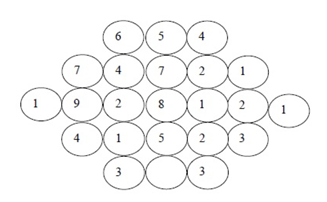
\includegraphics[]{figs/Q.8.png}
    \caption{}
    \label{fig:1}
\end{figure}


\hfill{(GATE AG 2015)}

\item 

A cube of side 3 units is formed using a set of smaller cubes of side 1 unit. Find the proportion of the number of faces of the smaller cubes visible to those which are NOT visible.
\begin{multicols}{4}
\begin{enumerate}
    \item  1:4
    \item  1:3
    \item  1:2
    \item  2:3
\end{enumerate}
\end{multicols}
\hfill{(GATE AG 2015)}

\item 

Humpty Dumpty sits on a wall every day while having lunch. The wall sometimes breaks. A person sitting on the wall falls if the wall breaks.


Which one of the statements below is logically valid and can be inferred from the above sentences?

\begin{enumerate}
    \item  Humpty Dumpty always falls while having lunch
    \item  Humpty Dumpty does not fall sometimes while having lunch
    \item  Humpty Dumpty never falls during dinner
    \item  When Humpty Dumpty does not sit on the wall, the wall does not break
\end{enumerate}
\hfill{(GATE AG 2015)}

\subsection{Q.11 to Q.35 carry 1 mark each and Q.36 to Q.65 carry 2 marks each.}


\item The series represented by 
\begin{align*}
a_n &= \frac{n^2 - 2n}{3n^2 + n}
\end{align*}
is
\begin{multicols}{4}
\begin{enumerate}
    \item  convergent
    \item  divergent
    \item  asymptotic
    \item  oscillatory
\end{enumerate}
\end{multicols}
\hfill{(GATE AG 2015)}

\item Inverse of the matrix 
\[
\myvec{3 & 2 \\ 1 & 4}
\]
is
\begin{multicols}{4}
\begin{enumerate}
    \item  $\myvec{0.1 & -0.4 \\ -0.3 & 0.2}$
    \item  $\myvec{0.3 & -0.2 \\ -0.1 & 0.4}$
    \item  $\myvec{0.3 & -0.1 \\ -0.2 & 0.4}$
    \item  $\myvec{0.4 & -0.2 \\ -0.1 & 0.3}$
\end{enumerate}
\end{multicols}
\hfill{(GATE AG 2015)}

\item The distance $PQ$ between two position vectors 
\[
\vec{P} = -2\hat{i} + 3\hat{j} + 4\hat{k}, 
\quad \vec{Q} = 4\hat{i} + 5\hat{j} + 7\hat{k}
\]
is $\_\_\_\_$.

\item The incorrect statement from the following is

\begin{enumerate}
    \item  The peak runoff from an agricultural watershed is generally less than that from an urban watershed of the same area
    \item  The horizontal hydraulic conductivity of soil is less than its vertical hydraulic conductivity
    \item  The magnitude of a 75-year flood is less than that of a 100-year flood
    \item  The rating curve due to an unsteady flood event forms a loop
\end{enumerate}
\hfill{(GATE AG 2015)}


\item If x be the highest mean monthly precipitation and y be the mean annual precipitation, then the 'rainfall aggressiveness' to soil erosion is
\begin{multicols}{4}
\begin{enumerate}
    \item  $\dfrac{x^2}{y}$
    \item  $\dfrac{x}{y^2}$
    \item  $\dfrac{x^2}{y^2}$
    \item  $\dfrac{y^2}{x}$
\end{enumerate}
\end{multicols}
\hfill{(GATE AG 2015)}

\item Discharge through an irrigation outlet is independent of the water levels in the distributary and water courses in case of 
\begin{multicols}{4}
\begin{enumerate}
    \item non-modular outlet
    \item semi-modular outlet
    \item Kennedy's gauge outlet
    \item Gibb's module outlet
\end{enumerate}
\end{multicols}
\hfill{(GATE AG 2015)}

\item The USDA classification of irrigation water with regard to alkali and salinity hazards is based on  
\begin{enumerate}
    \item Exchangeable sodium percentage and pH
    \item Electrical conductivity and Sodium adsorption ratio
    \item Electrical conductivity and pH
    \item Sodium percentage and pH
\end{enumerate}
\hfill{(GATE AG 2015)}

\item A steady discharge of $60 \, \text{m}^3 \text{s}^{-1}$ is passing through a trapezoidal irrigation channel with a bottom width of 5 m, bed slope of 0.01\% and Manning's roughness coefficient of 0.025. The conveyance of the channel in $\text{m}^3 \, \text{s}^{-1}$ is \_\_\_\_\_.  
\hfill{(GATE AG 2015)}

\item Dupuit-Forchheimer assumptions are used for analyzing groundwater flow in  
\begin{multicols}{4}
\begin{enumerate}
    \item confined aquifers
    \item leaky confined aquifers
    \item unconfined aquifers
    \item both confined and unconfined aquifers
\end{enumerate}
\end{multicols}
\hfill{(GATE AG 2015)}

\item An unsteady time-drawdown pumping test was conducted in a confined aquifer and the drawdown was measured with time in an observation well located at a certain distance away from the pumping well. Using these time-drawdown data, we can determine
\begin{multicols}{2}
\begin{enumerate}
    \item transmissivity only
    \item storage coefficient only
    \item specific storage only
    \item both transmissivity and storage coefficient
\end{enumerate}
\end{multicols}
\hfill{(GATE AG 2015)}

\item Mole drain is the most suitable drainage system for
\begin{multicols}{4}
\begin{enumerate}
    \item heavy clay soil
    \item loamy soil
    \item sandy soil
    \item silty soil
\end{enumerate}
\end{multicols}
\hfill{(GATE AG 2015)}

\item The efficiency of a cyclone separator can be increased by
\begin{multicols}{2}
\begin{enumerate}
    \item decreasing the size of the particles
    \item increasing the velocity of inlet air
    \item reducing the length of the separator
    \item reducing the diameter of air outlet
\end{enumerate}
\end{multicols}
\hfill{(GATE AG 2015)}

\item The correct statement in respect of rice parboiling process is
\begin{multicols}{2}
\begin{enumerate}
    \item kernel structure becomes soft and it cooks easily
    \item heat treatment during parboiling preserves some antioxidants
    \item parboiled rice retains more proteins, vitamins and minerals
    \item shelling of parboiled rice becomes more difficult
\end{enumerate}
\end{multicols}
\hfill{(GATE AG 2015)}

\item In the design of an agitator vessel with model volume $V_1$ and prototype volume $V_2$, the scale-up ratio is given by
\begin{multicols}{2}
\begin{enumerate}
    \item $\dfrac{V_2}{V_1}$
    \item $\left(\dfrac{V_2}{V_1}\right)^{1/2}$
    \item $\left(\dfrac{V_2}{V_1}\right)^{1/4}$
    \item $\left(\dfrac{V_2}{V_1}\right)^{1/3}$
\end{enumerate}
\end{multicols}
\hfill{(GATE AG 2015)}

\item 
The wall of a cold storage is made up of four layers; concrete, brick, cardboard and paint with respective thickness of 5, 60, 8 and 1 mm, and their corresponding thermal conductivities are 0.8, 0.7, 0.04 and 0.15 W m$^{-1}$ K$^{-1}$. The overall resistance of the wall to conduction heat transfer in m$^{2}$ K W$^{-1}$ is \_\_\_\_.
\hfill{(GATE AG 2015)}

\item 
Two very large parallel walls (gray bodies) facing each other have emissivities of 0.5 and 0.7. The view factor between these two walls is \_\_\_\_.
\hfill{(GATE AG 2015)}

\item 
In a counter-current flow double pipe heat exchanger (DPHE), temperature difference between the hot and cold liquids at all positions is held constant at C. If the effectiveness of the heat exchanger is 0.65 and heat capacity ratio of hot and cold liquids is 1, the number of transfer units (NTU) is \_\_\_\_.
\hfill{(GATE AG 2015)}

\item 
The values of $C$ and $n$ for raisin are $1.283 \times 10^{-4}$ K$^{-1}$ and 1.02, respectively in the Henderson equation. The equilibrium moisture content of raisin in percent dry basis corresponding to the air with 70\% relative humidity at 40 $^{\circ}$C is \_\_\_\_.
\hfill{(GATE AG 2015)}

\item 
A power operated chaff cutter with two knives is rotating at 600 rpm. It has a conveyor type feeding mechanism which operates at a speed of 0.6 m s$^{-1}$. The theoretical chaff length in mm is \_\_\_\_.
\begin{multicols}{4}
\begin{enumerate}
    \item 20
    \item 30
    \item 60
    \item 90
\end{enumerate}
\end{multicols}
\hfill{(GATE AG 2015)}

\item 
The conversion efficiency of a solar cell is 12\%. For a maximum power output of $9 \times 10^{-3}$ W at an incident solar radiation of 250 Wm$^{-2}$, the required surface area of the solar cell in mm$^{2}$ will be \_\_\_\_.
\hfill{(GATE AG 2015)}

\item 
The non-combustible constituents of the producer gas are
\begin{multicols}{2}
\begin{enumerate}
    \item Carbon monoxide and Hydrogen
    \item Hydrogen and Methane
    \item Nitrogen and Carbon dioxide
    \item Carbon monoxide and Nitrogen
\end{enumerate}
\end{multicols}
\hfill{(GATE AG 2015)}

\item 
The grain to straw ratio of wheat crop is 1.5 : 1. The output capacity and cleaning efficiency of a thresher at an optimal operating condition are 500 kg h$^{-1}$ and 99\%, respectively. If the grain recovery at main grain outlet is 100\%, the throughput capacity in kg h$^{-1}$ will be \_\_\_\_.
\begin{multicols}{4}
\begin{enumerate}
    \item 758
    \item 825
    \item 1238
    \item 1320
\end{enumerate}
\end{multicols}
\hfill{(GATE AG 2015)}

\item 
The brake power of a six-cylinder, four-stroke diesel engine running at 3000 rpm is 125 kW. Its brake specific fuel consumption is 200 g kW$^{-1}$ h$^{-1}$. Assuming specific gravity of fuel as 0.85, the volume of fuel to be injected per cycle per cylinder in ml is \_\_\_\_.
\hfill{(GATE AG 2015)}

\item 
For a reference sound pressure of $2 \times 10^{-5}$ N m$^{-2}$, the sound level measured at the operator's workspace of a tractor was 80 dB. If the RMS sound pressure is increased by eight times, the resulting sound pressure level in dB, will be \_\_\_\_.
\hfill{(GATE AG 2015)}

\item 
The connecting rod of an internal combustion engine is subjected to
\begin{multicols}{2}
\begin{enumerate}
    \item compression only
    \item tension only
    \item both compression and tension
    \item torsion only
\end{enumerate}
\end{multicols}
\hfill{(GATE AG 2015)}

\item 
Values of the function
\begin{align*}
    y = \dfrac{1}{1+x^{2}} 
\end{align*}
are $y(0) = 1$; $y(1) = 0.5$; $y(2) = 0.2$; $y(3) = 0.1$; $y(4) = 0.0588$; $y(5) = 0.0385$; $y(6) = 0.027$. Using Simpson's one-third rule, the value of the integral 
\begin{align*}
    \int_{0}^{6} \dfrac{dx}{1+x^{2}}
\end{align*}
is \_\_\_\_.
\hfill{(GATE AG 2015)}

\item 
Daily sales figures for a week are shown in the bar chart given below. The mean daily sales and the standard deviation of the sample mean (integer value) are \_\_\_\_ and \_\_\_\_, respectively.

\begin{figure}[H]
    \centering
    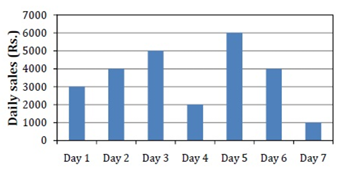
\includegraphics[]{figs/Q.37.png}
    \caption{}
    \label{fig:2}
\end{figure}

\begin{multicols}{2}
\begin{enumerate}
    \item 3571, 1718
    \item 3715, 1915
    \item 3571, 1178
    \item 3715, 1591
\end{enumerate}
\end{multicols}
\hfill{(GATE AG 2015)}

\item 
A coin is tossed ten times. The probability of getting five heads and five tails is \_\_\_\_.
\hfill{(GATE AG 2015)}

\item 
The particular solution to the first order differential equation 
\begin{align*}
\frac{dy}{dx} = x - e^{-x} \quad \text{for } y(0) = -1
\end{align*}
is \_\_\_\_.
\begin{multicols}{4}
\begin{enumerate}
    \item $2x^{2} + e^{-x} - 2$
    \item $2x^{2} + e^{-x} + \tfrac{1}{2}$
    \item $\tfrac{x^{2}}{2} - e^{-x} + \tfrac{1}{2}$
    \item $\tfrac{x^{2}}{2} + e^{-x} - 2$
\end{enumerate}
\end{multicols}
\hfill{(GATE AG 2015)}

\item 
The value of 
\begin{align*}
\int_{0}^{\pi/2} \sin^{3}x \, dx
\end{align*}
is \_\_\_\_.
\begin{multicols}{4}
\begin{enumerate}
    \item 0
    \item $\tfrac{1}{3}$
    \item $\tfrac{2}{3}$
    \item 1
\end{enumerate}
\end{multicols}
\hfill{(GATE AG 2015)}

\item 
Two irrigation channels are designed in the same type of alluvial soil having the channel bed slopes of $1.52 \times 10^{-4}$ and $1.6 \times 10^{-4}$, respectively. If the design discharge of the first channel, using Lacey's regime theory, is 30 m$^{3}$ s$^{-1}$, then the design discharge of the second channel in m$^{3}$ s$^{-1}$ will be \_\_\_\_.
\begin{multicols}{4}
\begin{enumerate}
    \item 22.05
    \item 29.74
    \item 30.26
    \item 40.81
\end{enumerate}
\end{multicols}
\hfill{(GATE AG 2015)}

\item 
A catchment of 720 ha area has 25-year mean rainfall intensity of 100 mm h$^{-1}$ occurring for a duration equal to its time of concentration. During a storm event, the catchment received a total of 7.5 cm design rainfall for 6 hours. Assuming $\phi$-index of 0.25 cm h$^{-1}$ and runoff coefficient of 0.6, the peak ordinate of the 6-h unit hydrograph in m$^{3}$ s$^{-1}$ will be \_\_\_\_.
\hfill{(GATE AG 2015)}

\item 
A Cipolletti weir has the crest length of 1.2 m and a crest water level of 0.5 m. The average approach velocity of water in m s$^{-1}$ on the crest is \_\_\_\_.
\begin{multicols}{4}
\begin{enumerate}
    \item 0.49
    \item 1.18
    \item 1.19
    \item 1.32
\end{enumerate}
\end{multicols}
\hfill{(GATE AG 2015)}

\item 
Match the following items between \textbf{Column-I} and \textbf{Column-II} with the most appropriate combinations.

\begin{center}
\begin{tabular}{ll}
\textbf{Column-I} & \textbf{Column-II} \\
i) Direct runoff & 1) T-year rainfall depth \\
ii) Peak runoff & 2) Curve Number \\
iii) Tensiometer & 3) Aquifer \\
iv) Isoerodent map & 4) Rational formula \\
v) Isopluvial map & 5) 30-minute rainfall intensity \\
vi) Zone of saturation & 6) Field capacity \\
\end{tabular}
\end{center}
\begin{multicols}{2}
\begin{enumerate}
    \item i-4, ii-2, iii-6, iv-5, v-1, vi-3
    \item i-2, ii-4, iii-6, iv-5, v-1, vi-3
    \item i-4, ii-2, iii-6, iv-1, v-5, vi-3
    \item i-2, ii-4, iii-6, iv-1, v-5, vi-3
\end{enumerate}
\end{multicols}
\hfill{(GATE AG 2015)}

\item 
An unconfined aquifer covering an area of 50 ha has a hydraulic conductivity of 20 m day$^{-1}$ and specific yield of 12\%. After a significant rainfall event, the water table rises from 17 m to 14.5 m below the ground level. Assuming no abstraction and outflow of groundwater during the recharge period, the amount of groundwater recharge contributed by the rainfall in m$^{3}$ is \_\_\_\_.
\hfill{(GATE AG 2015)}

\item 
If an irrigation water source has the concentrations of Na$^{+}$, Ca$^{++}$ and Mg$^{++}$ as 28, 10 and 5 milliequivalents per litre, respectively, then the Sodium adsorption ratio of this water is \_\_\_\_.
\hfill{(GATE AG 2015)}

\item  
In a canal command, maize crop is grown in an area of 30 ha. The crop evapotranspiration (ET$_c$) of maize is 840 mm per season and the effective rainfall during growing season is 20 mm. It is irrigated with water having salinity of 1.1 dS m$^{-1}$ by a surface irrigation method. If the leaching efficiency of the field soil is 0.8 and the average soil salinity tolerated by the maize crop for 100\% yield is 1.7 dS m$^{-1}$, the depth of irrigation water in mm per season required to meet the seasonal ET$_c$ and leaching requirement will be \_\_\_\_.
\hfill{(GATE AG 2015)}

\item 
The depth of the impounded water in a 72 m long earthen dam is 6.2 m, while the tail water is 2.2 m deep. The hydraulic conductivity of the isotropic and homogeneous soil-fill of the dam is 0.53 m day$^{-1}$. Flow net method is used to estimate seepage wherein the number of flow channels is 6 and the number of potential drops is 21. The seepage rate through the dam in m$^{3}$ day$^{-1}$ is \_\_\_\_.
\hfill{(GATE AG 2015)}

\item 
A horizontal screw conveyer of 2.4 m length conveys wheat grain of bulk density 680 kg m$^{-3}$ and materials factor 1.2. The screw diameter, shaft diameter and pitch of the screw are 0.5, 0.15 and 0.4 m, respectively. If the screw is completely filled with grains and rotates at 60 rpm, the capacity of the screw conveyer in m$^{3}$ h$^{-1}$ and the actual power required in hp (approximately) are \_\_\_\_ and \_\_\_\_, respectively.
\begin{multicols}{4}
\begin{enumerate}
    \item 257, 2.8
    \item 258, 2.5
    \item 275, 1.9
    \item 396, 2.9
\end{enumerate}
\end{multicols}
\hfill{(GATE AG 2015)}

\item 
A suspension contains $3.6 \times 10^{5}$ spores of \textit{C. botulinum} having a D-value of 1.5 minute at 121.1 $^{\circ}$C and $8.5 \times 10^{6}$ spores of \textit{B. subtilis} having a D-value of 0.9 minute at the same temperature. The suspension is heated at a constant temperature of 121.1 $^{\circ}$C. The heating time needed in minutes for the suspension to obtain a survival probability of $10^{-3}$ for the most heat resistant organism in it is \_\_\_\_.
\hfill{(GATE AG 2015)}

\item 
Match the following items between \textbf{Column-I} and \textbf{Column-II} with the most appropriate combinations.  

\begin{tabular}{ll}
\textbf{Column-I} & \textbf{Column-II} \\
1) Microwave dryer & P) Cyclone separation \\
2) Spray dryer     & Q) Sublimation of water \\
3) Freeze dryer    & R) Dielectric drying \\
4) Drum dryer      & S) Drying of fruit pulp \\
\end{tabular}
\begin{multicols}{2}
\begin{enumerate}
    \item 1-Q, 2-S, 3-R, 4-P
    \item 1-R, 2-P, 3-Q, 4-S
    \item 1-R, 2-S, 3-Q, 4-P
    \item 1-Q, 2-S, 3-P, 4-R
\end{enumerate}
\end{multicols}
\hfill{(GATE AG 2015)}

\item 
A ball mill of 1.8 m diameter is loaded with steel balls each having a diameter of 6 cm. The rotational speed of the ball is kept at 75\% of the critical speed. The operational speed of the ball mill in rpm is \_\_\_\_.
\hfill{(GATE AG 2015)}

\item 
A fat globule of 1.5 $\mu$m diameter is rising up in a stagnant skim milk medium of 1005 kg m$^{-3}$ density and 1.5 cP viscosity. If the density of the fat globule is 915 kg m$^{-3}$, the steady rising velocity of the globule in $\mu$m s$^{-1}$ is \_\_\_\_.
\hfill{(GATE AG 2015)}

\item 
Two kg mass of air at 40~$^\circ$C with 0.023 kg water vapour per kg dry air is mixed with 3 kg mass of air at 20~$^\circ$C with 0.008 kg water vapour per kg dry air to produce 5 kg mass of air at 60\% relative humidity at 28~$^\circ$C. Assume all the streams are at normal atmospheric pressure (101.325 kPa). The saturation vapour pressure of water in kPa at 28~$^\circ$C is \_\_\_\_.  
\hfill{(GATE AG 2015)}

\item 
In a cascade refrigeration system, the COPs of the cooling cycle and cascade are 3.7 and 4.2, respectively. If tonnage (1 TR = 3.52 kW) of the cooling cycle is 15 and the cascade removes 70\% of the total heat rejected in the liquid receiver of the cooling cycle, then the powers required by the cooling and cascade compressors in hp are \_\_\_\_ and \_\_\_\_, respectively.  
\begin{multicols}{4}
\begin{enumerate}
    \item 67.07, 46.95  
    \item 52.08, 39.35  
    \item 19.13, 14.99  
    \item 14.27, 11.18  
\end{enumerate}
\end{multicols}
\hfill{(GATE AG 2015)}

\item 
A single effect long-tube evaporator has ten tubes each of 2.5 cm diameter and 6 m length. It concentrates pineapple juice from 18~Brix to 23~Brix. The feed rate into the evaporator is 557 kg h$^{-1}$ at the boiling point of 70~$^\circ$C (latent heat of vaporization = 2333.82 kJ kg$^{-1}$). Neglecting boiling point rise, the overall heat transfer coefficient in W m$^{-2}$ K$^{-1}$ for 12~$^\circ$C temperature gradient across the tube walls is \_\_\_\_.  
\hfill{(GATE AG 2015)}

\item 
In a plate freezer, the plate temperature is maintained at --25~$^\circ$C. Latent heat of crystallization is 335 kJ kg$^{-1}$, and the thermal conductivity and density of frozen meat are 1.25 W m$^{-1}$ K$^{-1}$ and 1060 kg m$^{-3}$, respectively. Assuming freezing point of deboned meat at 85\% water content on wet basis to be 0~$^\circ$C, the freezing time in minutes for 2 cm thick block of meat, kept between a pair of freezing plates, is \_\_\_\_.  
\hfill{(GATE AG 2015)}

\item 
The horizontal component of soil forces acting on the front gang of a right hand offset disc harrow in the directions parallel and perpendicular to the direction of motion are 8 kN and 3 kN, respectively. The corresponding forces on the rear gang are 6 kN and 7 kN, respectively. If the horizontal component of pull acts towards the left of the direction of motion, its magnitude in kN will be \_\_\_\_.  
\hfill{(GATE AG 2015)}

\item 
A two-wheel drive tractor is operating a mould board plough at an average speed of 4 km h$^{-1}$. The draft and the rear axle torque are found to be 30 kN and 25 kN m, respectively. If the rolling radius of traction wheel is 0.7 m and the wheel slip is 20\%, the tractive efficiency in percent will be \_\_\_\_.  
\begin{multicols}{4}
\begin{enumerate}
    \item 67.19  
    \item 46.71  
    \item 72.87  
    \item 84.00  
\end{enumerate}
\end{multicols}
\hfill{(GATE AG 2015)}

\item 
A power operated hydraulic sprayer operating at a pressure of 1.4 MPa has a boom with 11 nozzles spaced at 0.3 m interval. The input power of the pump is 1.5 kW and its mechanical efficiency is 75\%. If the nozzle diameter and the discharge coefficient are 2.4 mm and 0.5, respectively, the average jet velocity of the nozzles in m s$^{-1}$ is \_\_\_\_.  
\hfill{(GATE AG 2015)}

\item 
A propeller type wind turbine of 8 m diameter generates 4 kW electrical power. If the overall efficiency of power generation system is 32\% and the density of air is 1.2 kg m$^{-3}$, the average wind speed in m s$^{-1}$ is \_\_\_\_.  
\hfill{(GATE AG 2015)}

\item 
In a reciprocating type mower, the maximum inertia force of 2.2 kN along the pitman occurs at 35$^\circ$ crank angle and 25$^\circ$ pitman angle with the horizontal plane. The crank radius is 50 mm and the equivalent mass at the crankpin is 2.5 kg. If the crank rotates at 600 rpm, the resultant force passing through the crankpin in kN will be
\begin{multicols}{4}
  \begin{enumerate}
      \item 2.25
      \item 2.68
      \item 2.98
      \item 3.42
  \end{enumerate}
  \end{multicols}
\hfill{(GATE AG 2015)}

\item 
A multiple disc clutch is to transmit 15 kW at 750 rpm. The inner and outer radii of the friction surfaces are 60 mm and 100 mm, respectively. The coefficient of friction is 0.1 and the maximum allowable pressure is 350 kPa. Assuming uniform wear, the number of pair of contact surfaces required is \_\_\_.
\hfill{(GATE AG 2015)}

\item 
The speed reductions in the 1$^{\text{st}}$ low gear of a tractor gearbox and differential with final drive are 5:1 and 40:1, respectively. For the tractor developing 24 kW power at an engine rpm of 2000 with an overall power transmission efficiency of 80\%, the total torque in kN m available at the wheel axle will be
\begin{multicols}{4}
  \begin{enumerate}
      \item 22.92
      \item 28.64
      \item 16.54
      \item 18.33
  \end{enumerate}
  \end{multicols}
\hfill{(GATE AG 2015)}

  \item A double acting hydraulic cylinder has a bore of 200 mm with a piston rod of 140 mm diameter. The extend speed of the piston is 80 mm s$^{-1}$. If the flow rate of oil during retraction is same as that of the extending, the retract speed of the piston in mm s$^{-1}$ is \_\_\_.
\hfill{(GATE AG 2015)}



\end{enumerate}
\end{document}

